% !TEX root = ../../../main.tex
% 来源：中学数学实验教材·第一册（代数）
% 章节：因式分解与余式定理 / 辗转相除法
% 原始文件：5.tex，行 2979-3007
% 类型：tikz
% ---
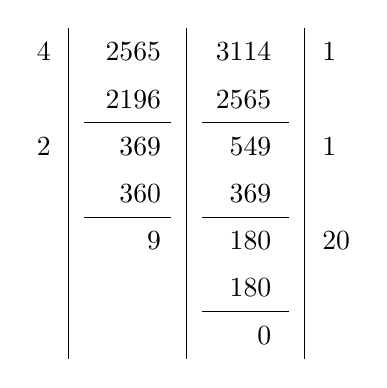
\begin{tikzpicture}[yscale=.6]
\foreach \x/\xtext in {6/2565, 5/2196, 4/369, 3/360, 2/\boxed{9}}
{
    \node at (-.2,\x)[left]{$\xtext$};
}

\foreach \x/\xtext in {6/3114, 5/2565, 4/549, 3/369, 2/180, 1/180, 0/0}
{
    \node at (1.2,\x)[left]{$\xtext$};
}

\foreach \x in {0,-1.5,1.5}
{
    \draw (\x, -.5)--(\x, 6.5);
}

\draw (-1.3, 4.5)--(-0.2, 4.5);
\draw (0.2, 4.5)--(1.3,4.5);
\draw (-1.3, 2.5)--(-0.2, 2.5);
\draw (0.2, 2.5)--(1.3,2.5);
\draw (0.2, .5)--(1.3,.5);

\node at (-1.6,6)[left]{4};
\node at (-1.6,4)[left]{2};
\node at (1.6,6)[right]{1};
\node at (1.6,4)[right]{1};
\node at (1.6,2)[right]{20};

\end{tikzpicture}    
